\documentclass[mathserif, aspectratio=169]{beamer}
\usetheme{odenpecos}
\setbeamertemplate{itemize/enumerate body begin}{\fontsize{8.8}{9}\selectfont}
\setbeamertemplate{itemize/enumerate subbody begin}{\fontsize{7.5}{8}\selectfont}
\setbeamertemplate{itemize/enumerate subsubbody begin}{\fontsize{7.5}{8}\selectfont}

% default search path for figures
\graphicspath{{./shared_figures/}{./fig/}}

\newcommand{\zapspace}{\topsep=0pt\partopsep=0pt\itemsep=0pt\parskip=0pt}

\usepackage{multicol}
\usepackage{pict2e}
%\usepackage{esdiff}
\usepackage{multimedia}
\usepackage{verbatim}
\usepackage{mhchem}
\usepackage{tikz}
\usetikzlibrary{arrows}


\usepackage[percent]{overpic}
\usepackage[absolute,overlay]{textpos}

\newcommand{\overbar}[1]{\mkern 1.5mu\overline{\mkern-1.5mu#1\mkern-1.5mu}\mkern 1.5mu}
\newcommand{\pp}[2]{\frac{\partial #1}{\partial #2}}
\newcommand{\dd}[2]{\frac{d #1}{d #2}}
\newcommand{\DD}[2]{\frac{D #1}{D #2}}
\newcommand{\mm}{\mathbf{minmod}}
\def\etal{{\it et al~}}
\newcommand{\be}{\begin{eqnarray}}
\newcommand{\ee}{\end{eqnarray}}
\newcommand{\mbb}[1]{\mathbb{#1}} % math blackboard bold
\newcommand{\mcal}[1]{\mathcal{#1}} % math blackboard bold
\newcommand{\mbf}[1]{\mathbf{#1}} % math bold face (for vectors)
\newcommand{\sbf}[1]{\boldsymbol{#1}} % bold face for symbols
\newcommand{\jump}[1]{\llbracket #1 \rrbracket} % jump operator
\newcommand{\avg}[1]{\langle #1 \rangle} % average operator
\newcommand{\rarrow}{\rightarrow}
\newcommand{\Rarrow}{\Rightarrow}
\newcommand{\LRarrow}{\Leftrightarrow}
\newcommand{\vvvert}{|\kern-1pt|\kern-1pt|}
\newcommand{\enorm}[1]{\vvvert #1 \vvvert}
\newcommand{\nutil}{\tilde{\nu}}
\newcommand{\Var}{\mathrm{Var}}
\newcommand{\Cov}{\mathrm{Cov}}


\definecolor{MyDarkGreen}{rgb}{0,0.45,0.08}
\newcommand{\myred}[1]{{\color{red} #1}}
\newcommand{\myblue}[1]{{\color{blue} #1}}
\newcommand{\mygreen}[1]{{\color{MyDarkGreen} #1}}

\newcommand{\sa}{\nu_{\mathrm{sa}}}
\newcommand{\tep}{\tilde{\epsilon}}
\newcommand{\Ssd}{\mathcal{S}} % source term due to slow derivative
\newcommand{\ud}{\,\mathrm{d}}

\newcommand{\Mach}[1]{\ensuremath{\mbox{Ma}_{#1}}}
\newcommand{\Reynolds}{\ensuremath{\mathit{Re}}}
\newcommand{\DensityRat}{\ensuremath{\mathit{DR}}}
\newcommand{\BlowRat}{\ensuremath{\mbox{BR}}}
\newcommand{\VelRat}{\ensuremath{\mathit{VR}}}
\newcommand{\Tau}{\ensuremath{\mathrm{T}}}

\newcommand{\wall}     {\ensuremath{\mathrm{w}}}   % wall subindex
\newcommand{\awall}    {\ensuremath{\mathrm{aw}}}  % adiabatic wall subindex

\newcommand{\commentout}[1]{}

\newcommand{\vect}[1]{\boldsymbol{#1}}
\usepackage{mleftright}
\newcommand{\of}[1]{\mleft( #1 \mright)}
\newcommand{\vth}{v_{\textrm{th}}}
\newcommand{\reals}{\mathbb{R}}
\newcommand{\myint}{\int\limits}
\newcommand{\ddt}[1]{\partial_t #1}
\newcommand{\RR}{\mathbb{R}}
\newcommand{\vr}{v}
\newcommand{\diff}[1]{\, d#1}
\newcommand{\norm}[1]{\left\lVert#1\right\rVert}
%\newcommand{\vtheta}{\theta_{\vect{v}}}
%\newcommand{\vphi}{\varphi_{\vect{v}}}
%\newcommand{\vr}{v_{r}}
\newcommand{\vtheta}{{v_{\theta}}}
\newcommand{\vphi}{v_{\varphi}}
\newcommand{\vomega}{v_{\omega}}
\newcommand{\vrunit}{\hat{\vect{v}}_{r}}
\newcommand{\vthetaunit}{\hat{\vect{v}}_{\theta}}
\newcommand{\vphiunit}{\hat{\vect{v}}_{\varphi}}
\DeclareMathOperator{\variance}{Var}

\begin{document}
% disable nav
\setbeamertemplate{navigation symbols}{}

% ---------------------------------------------------------------
% Oden/Pecos title page

%\hoffset=.16in
%
\begin{frame}[plain,t]{}
\makeatletter
%\vspace*{0.85cm}
%\vspace*{0.65cm}
\includegraphics[height=0.9in,trim=50 40 40 0, clip]{PMSc_159_university_formal_horizontal.pdf} \newline
%\vspace*{0.3cm}
\begin{columns}[T,onlytextwidth]
\column{.8\textwidth}
{\bf \color{burntorange} \fontfamily{bch}\selectfont 
% -- Set talk title here
Solving the Boltzmann equation for electron kinetics using Petrov-Galerkin approach
% --
}
\end{columns}
\vspace*{.15cm}
\rule{.8\textwidth}{0.6pt} \newline

\vspace*{0.05cm}
\setstretch{0.65}
{\fontfamily{phv}\selectfont
  { \scriptsize
    % -- define presenter, authors here
    Milinda Fernando, Daniil Bochkov, Todd Oliver, Raja Laxminarayan, Philip Varghese, Bob Moser, George Biros\newline
    % --
  }
  {\color{burntorange} \tiny
    % -- define role, meeting event, location, etc
    %Year-1 Review $\cdot$ August, 2021 $\cdot$ Austin, TX
    All-hands Meeting $\cdot$ July, 2022 $\cdot$ Austin, TX
    % --
  }
}

\vspace*{1cm}
%\includegraphics[height=0.3in]{figures/pecos_orange1.png}
\begin{columns}
\begin{column}{0.8\linewidth}
\includegraphics[height=0.5in]{oden_pecos_2020_wordmark.png}\\
{\scriptsize \url{https://pecos.oden.utexas.edu}}
\end{column}

\begin{column}{0.2\linewidth}
\includegraphics[height=0.6in]{psaap3-logo.png}
\end{column}
\end{columns}

\end{frame}
\hoffset=0in
% -- end title slide ---------------------------------------------

\begin{frame}
	\frametitle{Boltzmann Equation}
\begin{itemize}
	\item The Boltzmann equation describes the evolution of the electron distribution function $f=f(\vect{x}, \vect{v}, t)$. %Electron distribution function defines the transport and kinetic properties, and its evolution is described by the Boltzmann equation.
	\begin{align}
		\partial_t f + \vect{v}\cdot \nabla_{\vect{x}} f  + \frac{\vect{E} q}{m} \cdot \nabla_{\vect{v }}f = C(f)
	\end{align}
	\item Challenges : 6+1 dimensions, accurate tail representation of $f$
	\item \textbf{For this work}: We focus only velocity-space discretization (i.e., spatially homogeneous case, $f=f(\vect{v}, t)$) 
	\item \textbf{Explore}: Global and localized approximations of $f$ with Maxwell and B-splines. 
\end{itemize}
\end{frame}

\begin{frame}
	\frametitle{Petrov-Galerkin approach}
	\small
	\begin{itemize}
		\item Weak formulation:
		$
		\displaystyle
		\quad
		\partial_t f + \frac{\vect{E} q}{m} \cdot \nabla_{\vect{v}}f = C(f)
		\quad \rightarrow \quad
		\partial_t \myint_{R^3} f \phi\of{\vect{v}} \ud \vect{v} = 
		\myint_{R^3} C(f) \phi\of{\vect{v}} \ud \vect{v} - \myint_{R^3} \of{\frac{\vect{E} q}{m} \cdot \nabla_{\vect{v}} f} \phi(\vect{v}) \ud\vect{v}
		$

		\item $f$ is approximated as isotropic + anisotropic correction terms.
		$
		\displaystyle
		\quad 
		f(\vect{v},t) = M(v)\sum_{klm} f_{klm} \Phi_k\of{v} Y_{lm}\of{v_\theta, v_\phi}$ with $
		\displaystyle
		\quad 
		\phi_{pqs}\of{\vect{v}} = \underbrace{\Phi_p\of{v}}_{\text{radial basis}} \underbrace{Y_{qs}\of{v_\theta, v_\phi}}_{\tiny\text{sph. harm.}}$

		\item Resulting system of ODEs, 
		$ \displaystyle
		\quad 
		\sum_{k,l,m} M_{p,q,s}^{k,l,m} \partial_t h_{k,l,m}\of{t} = \sum_{k,l,m}  \of{\underbrace{C_{p,q,s}^{k,l,m}}_{\text{collision op.}}  - \underbrace{E_{p,q,s}^{k,l,m}}_{\text{advection op.}}} h_{k,l,m}\of{t}$
		\item \textbf{Discretized operators}: For $N_r, N_{lm}$ be number of basis functions used in radial and angular directions, then matrices are $(N_rN_{lm} \times N_rN_{lm})$.
	\end{itemize}
\end{frame}

\begin{frame}
	\frametitle{Investigation of different bases}
	\begin{itemize}
		\item Choice of basis functions in radial direction
		\begin{itemize}
			\item Global approximations with global polynomials
			\item Local approximations with B-Splines with local support 
		\end{itemize}
	\end{itemize}
		\small
		\begin{align*}
		\textrm{Assoc. Laguerre poly:}
		& \quad \Phi_n\of{v} = L_n\of{v^2}, &&
		\quad 
		\myint_{0}^{+\infty} v^2 e^{-v^2} L_n\of{v^2} L_{n^\prime}\of{v^2} \ud v \sim \delta_{nn^\prime}
		\\
		\textrm{Maxwell (speed) poly:}
		& \quad \Phi_n\of{v} = P_n\of{v}, &&
		\quad 
		\myint_{0}^{+\infty} v^2 e^{-v^2} P_n\of{v} P_{n^\prime}\of{v} \ud v \sim \delta_{nn^\prime}
		\\
		\textrm{B-Splines:}
		& \quad \Phi_n\of{v} = B_n\of{v}, &&
		%\quad 
		%N_n\of{v} = 1 - \frac{|x-x_n|}{\Delta x},\quad x_{n-1} < x < x_{n+1}
		\end{align*}	
\end{frame}

\begin{frame}[fragile]
	\frametitle{Collision operator}
	\begin{itemize}
		\item Describes the underlying collisions. Currently consider electron-heavy particle collisions. 
		\item For binary collisions assuming $f_o(\vect{v},t)=n_o \delta(\vect{v})$ for heavy species (i.e., $n_o$ heavy species number density). \\
		$	\displaystyle
			\quad
			\myint_{R^3}{} C \phi\of{\vect{v}} \diff{\vect{v}} 
			=
			n_0 \myint_{R^3}{} \myint_{S^2}{} 
			B\of{\vect{v}, \vect{\omega}} 
			f\of{\vect{v}}
			\left(
			\phi\of{\vect{v}^\text{post}\of{\vect{v},\vect{\omega}}} 
			- \phi\of{\vect{v}} 
			\right)
			\diff{\vect{v}} \diff{\vect{\omega}}$
		\item Collision probability kernel $B\of{\vect{v}, \vect{\omega}}=\norm{\vect{v}} \underbrace{\sigma(\norm{\vect{v}}, \vect{\omega})}_{\text{LXCAT experimental data}}$
		\item We consider the following collisions. 
		\begin{itemize}
			\item G0 : $e + A \rightarrow e + A$ 
			\item G2 (ionization) : $e + A \rightarrow 2e + A^+$ 
		\end{itemize}
		\item We use \texttt{numpy} contractions for efficient computation of $C(f)$ (i.e., 5d quadrature with grid sizes of $256\times 4\times 4 \times 4 \times 4$). 
	\end{itemize}
\end{frame}

\begin{frame}
	\frametitle{Collision cross-sections}
	\begin{itemize}
		\item Get experimental cross-section data from LXCAT database (\text{https://nl.lxcat.net/home/}). 
		\item We observed slower convergence rate with direct sampling of LXCAT data. 
		\item To avoid above and other numerical instabilities, we use \textbf{curve-fitted} LXCAT data% (i.e., approximate LXCAT cross-sections with smooth functions).
	\end{itemize}
	\begin{center}
		\begin{tabular}{cc}
			$e + Ar \rightarrow e + Ar $ & $e + Ar \rightarrow 2e + Ar^+ $ \\
			\includegraphics[width=0.36\textwidth]{fig/g0.png} &  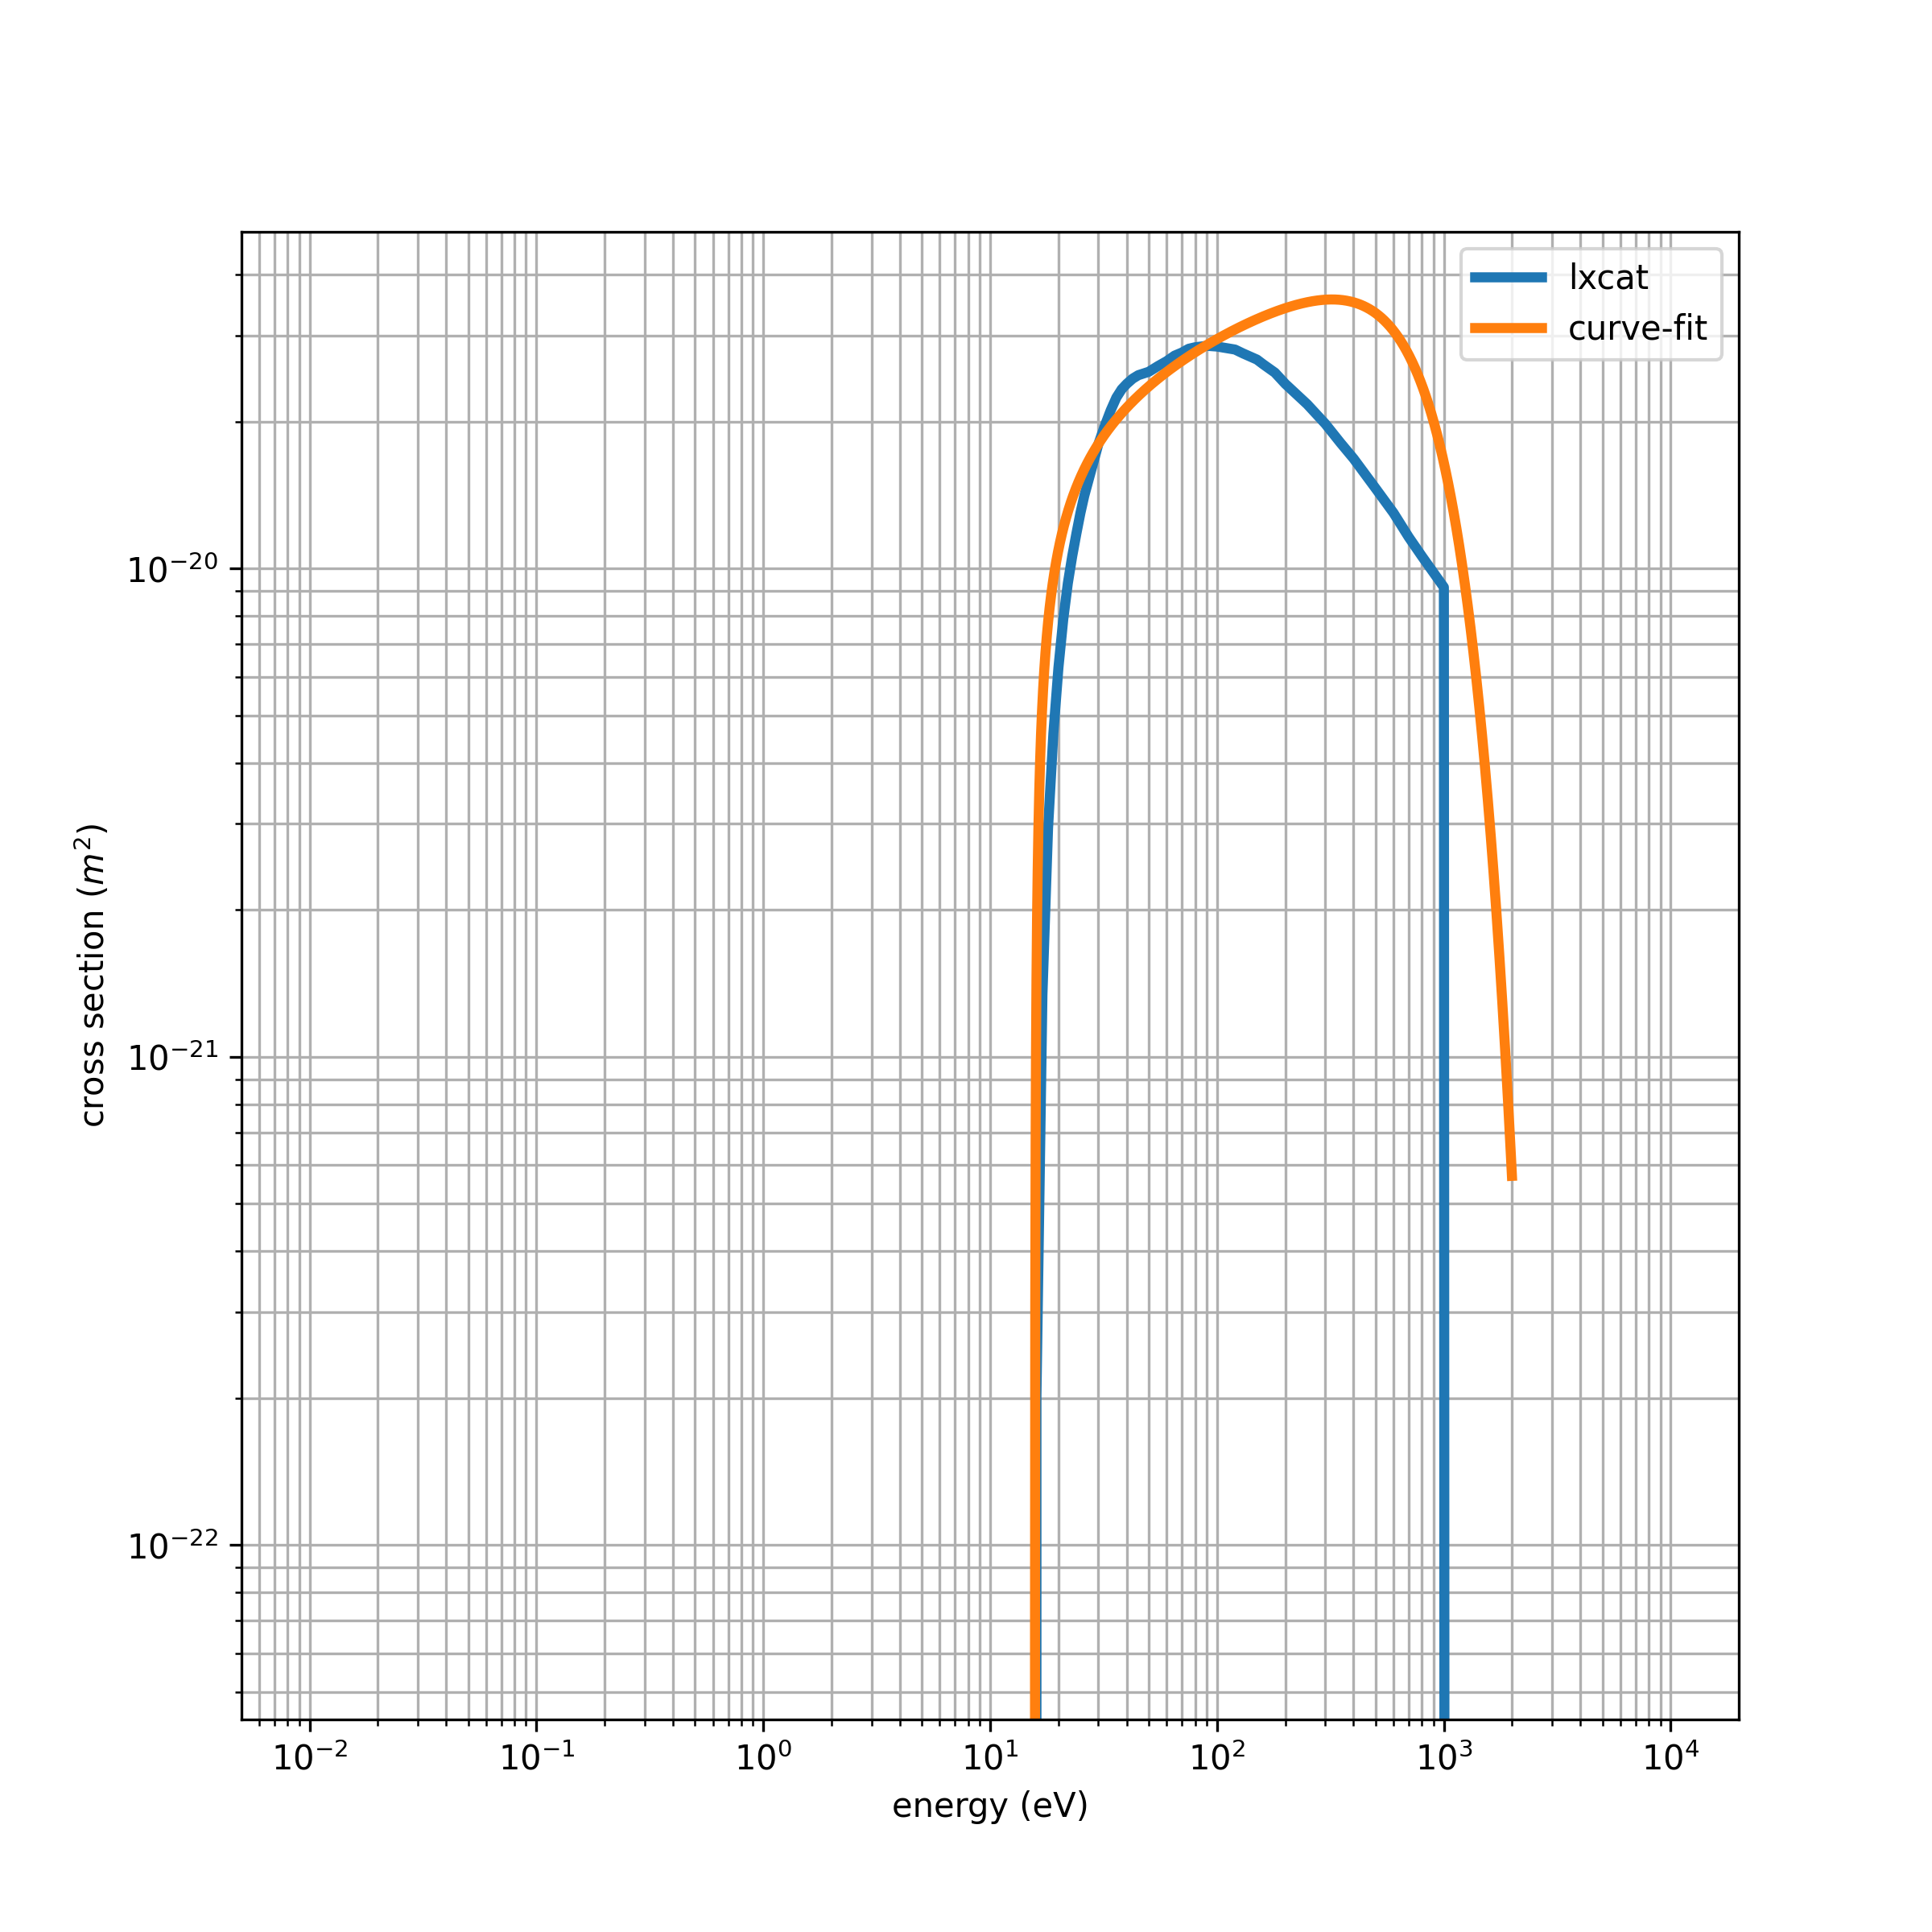
\includegraphics[width=0.36\textwidth]{fig/g2.png}
		\end{tabular}	
	\end{center}
\end{frame}

\begin{frame}
	\frametitle{Steady-state solution}
	\begin{itemize}
		\item $\frac{\vect{E} q}{m} \cdot \nabla_{\vect{v}}f$ acceleration of electrons due to the $E$ field (i.e., adds energy to system), $C(f)$ causes to lose energy due to collisions. 
		\item With $\vect{E}\neq 0$, the normalized distribution function should reach a steady state. Note: Ionization does not preserve mass (i.e., $n_e(t)=\myint_{R^3} f(\vect{v},t) \diff{\vect{v}}$).
		$
		\displaystyle
		\quad
		\partial_t (\hat{f}) = -(u^T C \hat{f}) \hat{f} + (C-E)\hat{f} \text{ where } \hat{f}(\vect{v},t) = \frac{f(v,t)}{\myint_{R^3} f(\vect{v},t) \diff{\vect{v}}}
		$
		\item Numerical evolution of the normalized distribution result in a DAE with constraint $u^T \hat{f}-1=0 \forall t>0$
		\item Steady-state solution to the above can be achieved via solving below.  
		$
		\displaystyle
		\quad
		\partial_t (\hat{f}) = 0 \Rightarrow -(u^T C \hat{f}) \hat{f} + (C-E)\hat{f} =0
		$ with $u^T \hat{f}-1=0$
		\item For the work presented, we use steady-state solve, avoiding time integrator to reach the steady-state solution. 
	\end{itemize}
\end{frame}

\begin{frame}
	\frametitle{Simplifying the collision operator}
\begin{itemize}
	\item For the moment assume lm=(0,0), (1,0) modes, (i.e., two term expansion of distribution function)
	\item $\vect{v}^{\prime} = (v_r^\prime, v_\theta^\prime, v_\phi^\prime) =\vect{v}^{post}\of{\vect{v},\vect{0},\vect{\omega}}$
	\begin{align*}
		\cos v_\theta^\prime = \cos v_\theta \cos\chi + \sin v_\theta \sin \chi \cos\of{v_\phi-\phi}
	\end{align*}
	\item Using the spherical harmonics addition theorem, we can write. 
	\begin{align*}
		P_l^{0} = P_l\of{\cos v_\theta^\prime} =  P_l\of{\cos v_\theta} P_l\of{\cos v_\phi} + 2\sum_{m=1}^{l} P_l^{m}\of{\cos v_\theta} P_l^{m}\of{\cos v_\phi} \cos \of{ m (v_\phi-\phi)}
	\end{align*}
	\item Analytically integrating out the angles, we can write,
	\begin{align*}
		C^{pq0}_{kl0}  = n_0 v_{th}^3 \myint_{R} x^2 B(x v_{th}) S_k\of{x} \delta_{ql} \of{T_p\of{x^\prime}\delta_{q0} - T_p\of{x}} \diff{x}  
	\end{align*}
\end{itemize}
\end{frame}

\begin{frame}
	\frametitle{EEDF formulation}
	\begin{itemize}
		\item Projecting only for the spherical basis, we can write, 
		\begin{align*}
			\frac{d}{dt} f_{0,0} - E 
			\left( \frac{1}{\sqrt{3}} \frac{d}{d\vr} f_{1,0} 
			+  \frac{2}{\sqrt{3}} \frac{1}{\vr} f_{1,0} \right) &= \tilde{C}^{00}_{00} f_{0,0} = \tilde{C_0} f_{0,0}
			\\
			\frac{d}{dt} f_{1,0} - E 
			\left( \frac{1}{\sqrt{3}} \frac{d}{d\vr} f_{0,0} \right) &=  \tilde{C}^{10}_{10} f_{1,0} = \tilde{C_1} f_{1,0}
		\end{align*}
		\item Based on the weak form of the $C^{10}_{10}$, 
		\tiny 
		\begin{align*}
		C^{10}_{10} = -n_0 v_{th}^4 \myint_{R} x^3 \sigma\of{\varepsilon} S(x) T(x) dx \implies  \tilde{C}^{10}_{10} = -n_0 \varepsilon^{1/2} \gamma \sigma\of{\varepsilon} 
		\end{align*} Let $\mu = \cfrac{\dot{n}_e}{n_e}$ be the growth rate due to collisions. In the weak form, 
		\begin{align*}
		&n_e\of{t} =\myint_{\vect{V}} f(t,v) \diff{\vect{v}} \\
		&\partial_t f(t,v) = C f \implies \mu = \frac{\dot{n}_e\of{t}}{n_e\of{t}} = \myint_{\vect{V}} C f \diff{\vect{v}} = u^T C \hat{f} \text{ where } \hat{f} = f/n_e
		\end{align*}
	\end{itemize}
\end{frame}

\begin{frame}
	\frametitle{EEDF formulation}
	\begin{itemize}
		\item For steady state we can write, 
		\begin{align*}
			&\partial_t \hat{f_1} = \frac{1}{n_e} \partial_t f_1 - \frac{\dot{n_e}}{n_e} \hat{f_1} =0 \implies 
			&\hat{f_1} = \frac{E}{\sqrt{3}} \frac{\partial_{v}\hat{f_0}}{(n_0 \varepsilon^{1/2}\gamma \sigma\of{\varepsilon} + \mu)}
		\end{align*}
		\begin{align*}
			&\partial_t \hat{f_0} = \frac{1}{n_e} \partial_t f_0 - \mu \hat{f_0} = 0  \implies
			&\frac{E^2}{3} \partial_{v} \of{\frac{\partial_v \hat f_0}{(n_0 \varepsilon^{1/2}\gamma \sigma\of{\varepsilon} + \mu)}} + \frac{2E^2}{3v} \frac{\partial_v \hat{f_0}}{(n_0 \varepsilon^{1/2}\gamma \sigma\of{\varepsilon} + \mu)} + \tilde C_0 \hat{f_0} = \mu \hat{f_0}\\
		\end{align*}
		\item Important to notice that we get a diffusion term in v-space. 
		\item Only solve for $\hat{f}_0$ and compute $\hat{f_1}$ from derivative of $\hat{f}_0$.
		\item Bolsig+ code use different electron-growth rate model than our formulation. 
	\end{itemize}
\end{frame}

\begin{frame}
	\frametitle{Numerical solutions: EEDF formulation}
	\begin{itemize}
		\item We can further simplify, and compute the discretized operators, 
		{\tiny
		\begin{align*}
			&W_{ij} = \Big[v^2 T(x) \frac{\partial_v \hat f_0}{(n_0 \varepsilon^{1/2}\gamma \sigma\of{\varepsilon} + \mu)}\Big]_0^{v_{max}}-\myint_{R} \frac{\partial_v S_j(x)}{(n_0 \varepsilon^{1/2}\gamma \sigma\of{\varepsilon} + \mu)} v^2 \partial_v T_i(x) dv \\
			&\myint_{R} v^2 \tilde{C}_0 dv = C_{0}  = n_0 v_{th}^3 \myint_{R} x^2 B(x v_{th}) S_k\of{x}  \of{T_p\of{x^\prime} - T_p\of{x}} \diff{x}  \\
			&M_{ij} = \myint_{R} v^2 T_i(x) S_j(x) dv\\
		\end{align*}}
		\item Therefore we can write, the residual functional and its Jacobian for the steady state which are used for non-linear solve. 
		\begin{align*}
			R(\hat{f_0}) &= C_0 \hat{f_0} + W^{\hat{f_0}}_{ij} (\hat{f_0}) - (u^T C_0 \hat{f_0}) M_{ij} \hat{f_0} \\
			J(\hat{f_0}) &= C_0 + W^{\hat{f_0}}_{ij}  - 2(u^T C_0 \hat{f_0}) M_{ij}
		\end{align*}
	\end{itemize}
\end{frame}

\begin{frame}
	\frametitle{\small Comparison with Bolsig with solving for $\hat{f}_0$ and $\hat{f}_1$}
	\begin{figure}
		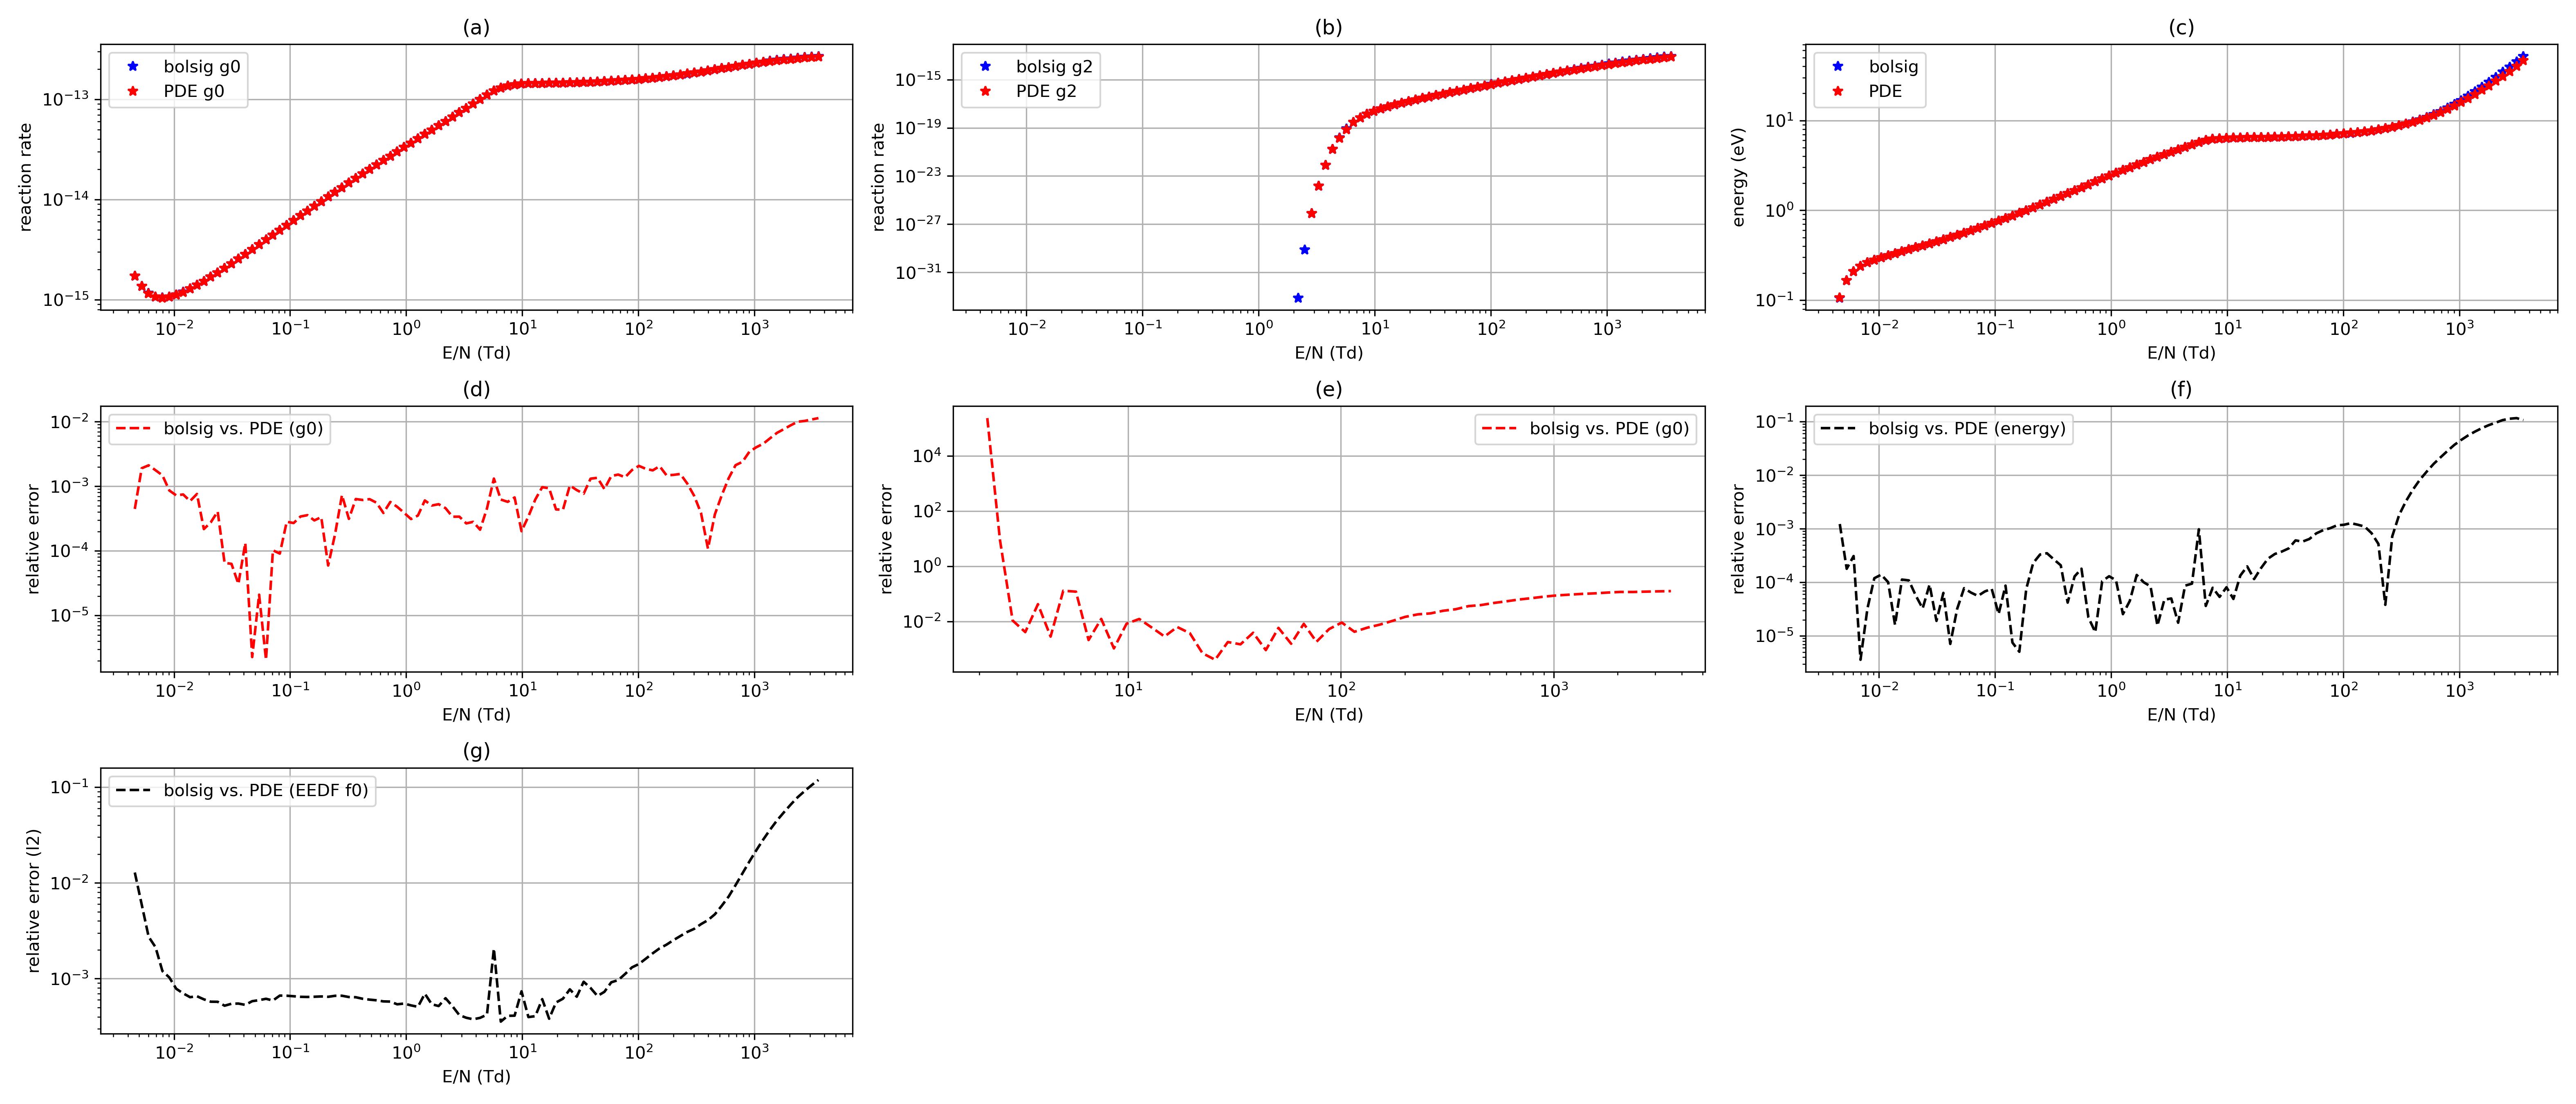
\includegraphics[width=\textwidth]{PDE_vs_BOLSIG_G0_G2.png}
	\end{figure}
\end{frame}


\begin{frame}
	\frametitle{\small Comparison with Bolsig with EEDF formulation}
	\begin{figure}
		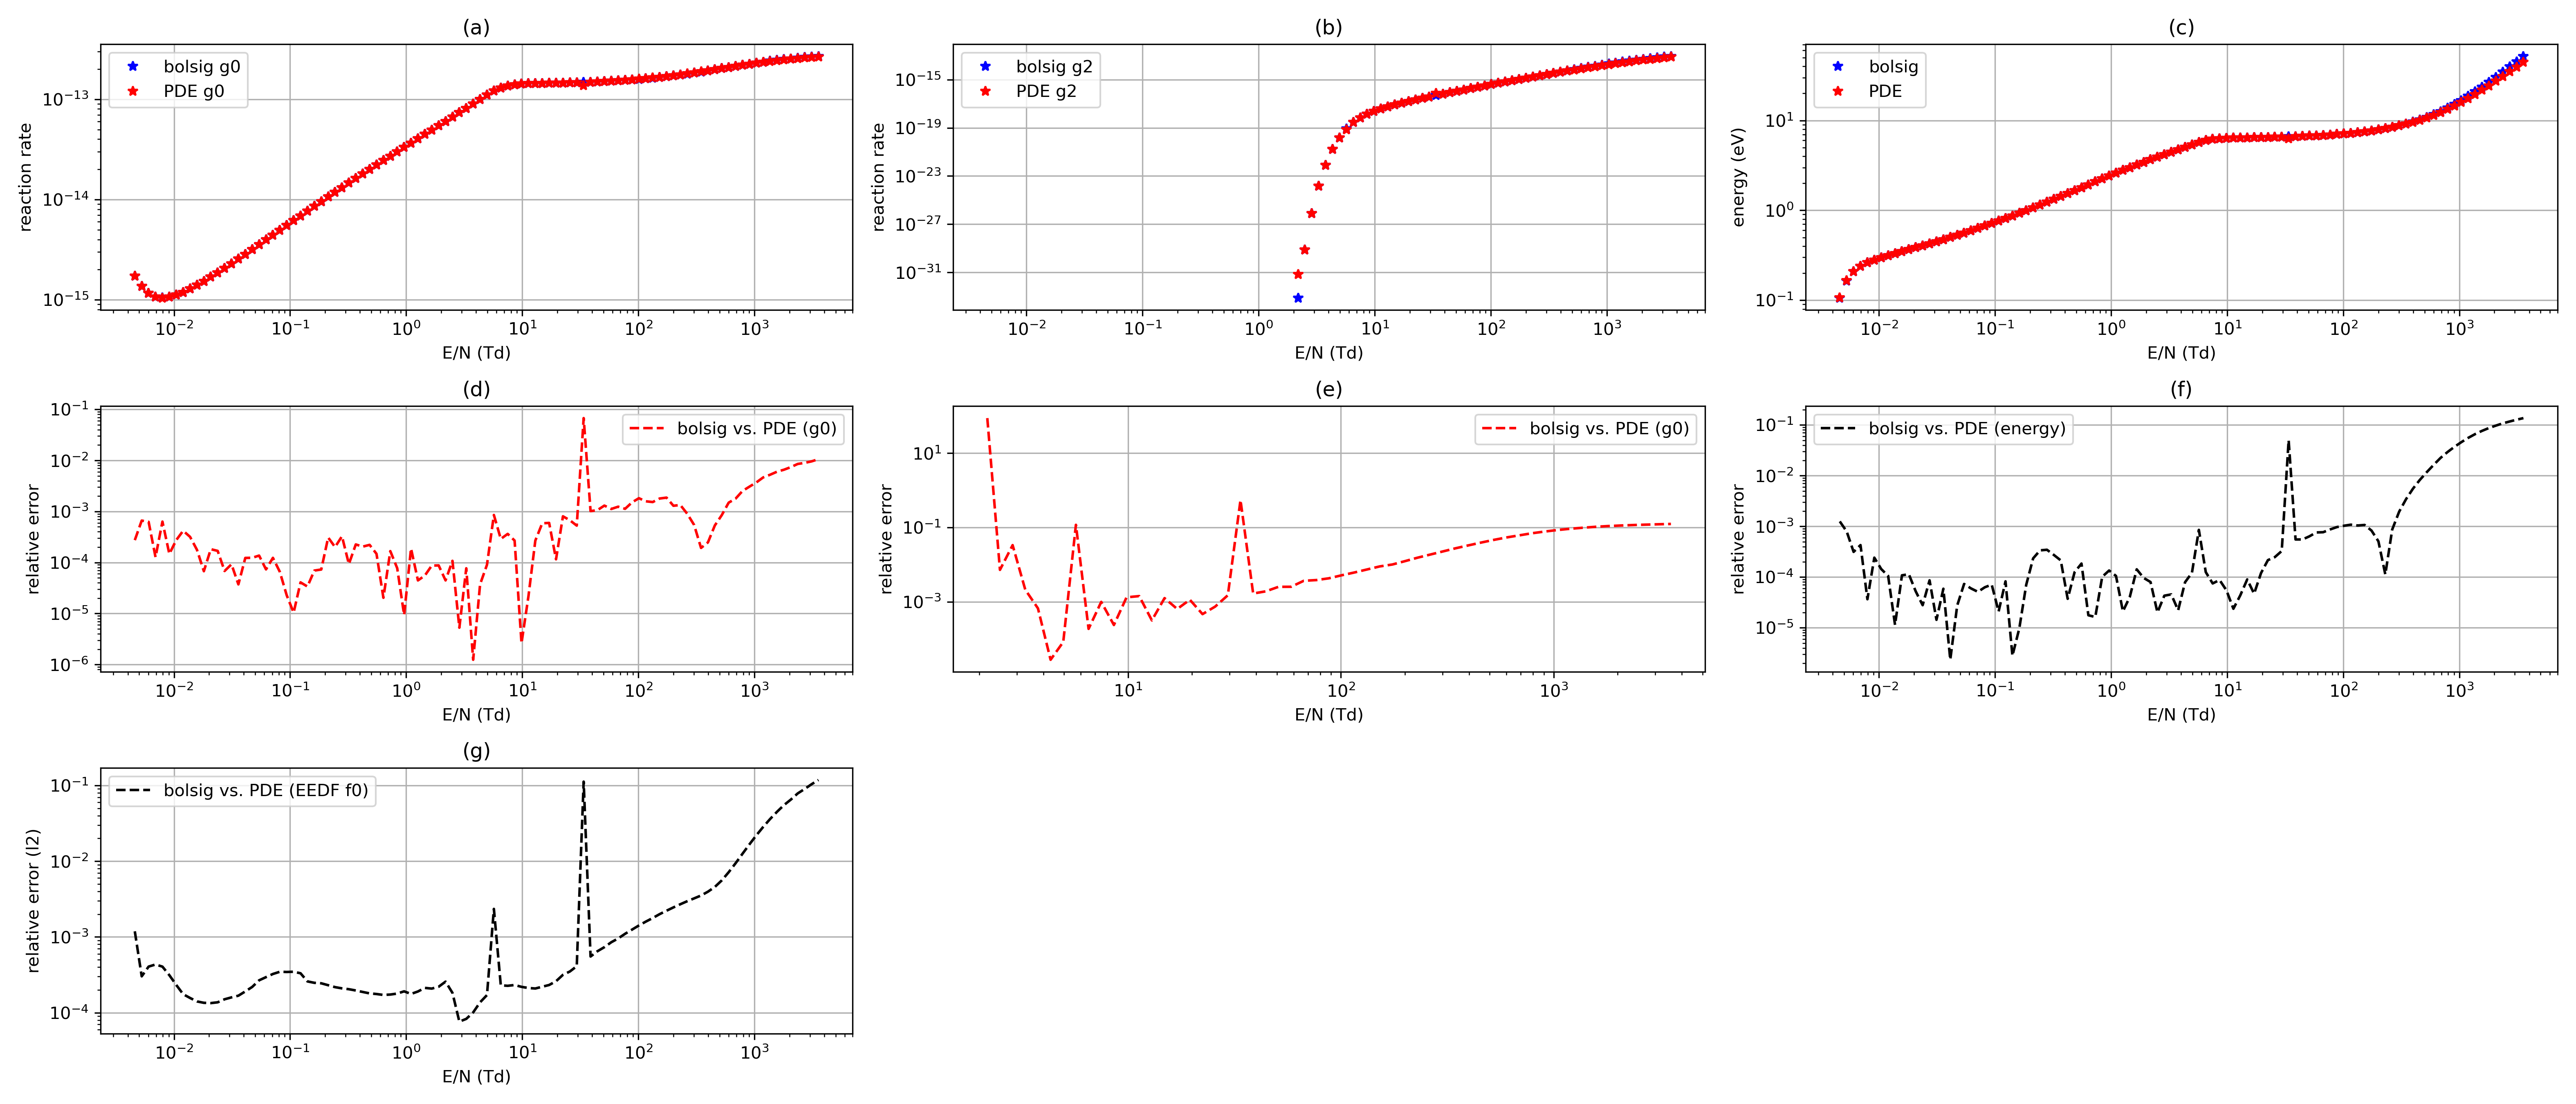
\includegraphics[width=\textwidth]{PDE_vs_BOLSIG_G0_G2_collop_approx.png}
	\end{figure}
\end{frame}

\begin{frame}
	\frametitle{EEDF Vs. two term formulation}
	\begin{figure}
		\only<+>{\includegraphics[width=\textwidth]{c_full_op1.png}}
		\only<+>{\includegraphics[width=\textwidth]{c_appx_op1.png}}
		\only<+>{\includegraphics[width=\textwidth]{c_full_op2.png}}
		\only<+>{\includegraphics[width=\textwidth]{c_appx_op2.png}}
	\end{figure}
\end{frame}


\begin{frame}
	\frametitle{1d glow discharge problem}
	\begin{itemize}
		\item The ionized heavy densities are governed by the drift-diffusion equation below.
			\begin{align*}
			&\partial_t n_i + \partial_z J_i = k_i n_0 n_e \text{ where } J_i\of{z, t} = \mu_i n_i E\of{z,t} -D_i \partial_z n_i\\
			&J_i(z,t)=\max\of{\mu_i n_i \vect{E}\cdot \vect{\hat{n}},0} \text{ for } z =0 \text{ and } z=L
			\end{align*}
		\item E-field is computed with 
			\begin{align*}
			\nabla V = -\frac{e}{\epsilon_0} (n_i-n_e) \text{ where } n_e(z,t) = \myint_{\vect{v}} f(\vect{v}, z, t) \diff{\vect{v}} \\
			V(0,t) = V_0 \sin(2\pi ft) \text{ , } V(L,t) = 0 \text{ and } \vect{E} = E \vect{\hat{z}} = -\of{\partial_z V} \vect{\hat{z}}
			\end{align*}
		\item 1d-space Boltzmann equation is given below. 
		\begin{align*}
			&	\partial_t f + v\cos\of{\vtheta} \partial_z f -\vect{E}\cdot\nabla_v f = C[f] \text{ for } (z,\vect{v}) \in (0,L) \times[0,v_{max}]^3 \\
			& f(\vect{v}, 0, t, \vtheta \leq \frac{\pi}{2})	= 0 \text{ and } f(\vect{v}, L, t, \vtheta > \frac{\pi}{2})	= 0
		\end{align*}
	\end{itemize}
\end{frame}

\begin{frame}
	\begin{center}
		\includegraphics[width=0.8\textwidth]{fig/glow_discharge_1d3v_g0_v0_z01.0_E0.0_poly_bspline_sp_2_nr128_qpn_4_ev2.000000E+00_bscale1.0_dt1.0000E-13_T1.00E-09_qoi.png}
	\end{center}
\end{frame}

%\begin{frame}
%	\frametitle{BTE boundary conditions}
%	\begin{itemize}
%		\item we use collocation method in $\vtheta$ and $z$ directions. 
%		\item Use projection operators to compute $l$ modes 
%	\end{itemize}
%	\begin{align*}
%		&f(v, \vtheta_j , z, t) = f_{\vtheta_j} (v, z, t) = \sum_k f_{\vtheta_j, k} \of{z,t} S_k\of{\frac{v}{\vth}} \\
%	\end{align*}
%
%	\begin{align*}
%		&	f_k\of{\vtheta,z,t} = \sum_l f_{lk}\of{z, t} Y_{l0}\of{\vtheta}\\
%		&	f_{lk} = 2\pi \myint_{\vtheta} \sin\of{\vtheta} f_k\of{\vtheta, z, t} Y_{l0} d\vtheta \\
%		&\sum_{\vtheta_j} w_{\vtheta_j} f_{\vtheta_j,k} Y_{l0}\of{\vtheta_j} = P^{\vtheta_j}_l f_{\vtheta_j,k}
%	\end{align*}
%	
%	\begin{align*}
%		\of{I_{N_\vtheta} \otimes M^{p}_{k}} \partial_t f_{\vtheta_j, k , z, t} + \of{I_{N_\vtheta} \otimes \of{\cos\of{\vtheta_j} W^{p}_k D_z}} f_{\vtheta_j, k , z, t} \\
%		= Y_{\vtheta_j, q} (E^{pq}_{kl} + C^{pq}_{kl}) \of{P^{\vtheta_j}_{l} f_{\vtheta_j,k,z,t}}^{T}
%	\end{align*}
%\end{frame}








\end{document}

